% --------------------------------------------------------------
% This is all preamble * that you don't have to worry about.
% Head down to where it says "Start here"
% --------------------------------------------------------------
 
\documentclass[12pt]{article}
 
\usepackage[margin=1in]{geometry} 
\usepackage{amsmath,amsthm,amssymb}
\usepackage{enumitem, blkarray}

\usepackage{hyperref, float, multicol, qtree, color, tkz-graph}
 
\newcommand{\lp}{\left(}
\newcommand{\rp}{\right)}
\newcommand\tline[2]{$\underset{\text{#1}}{\text{\underline{\hspace{#2}}}}$}
\newcommand\fline[2]{$\underset{\text{#1}}{\text{\underline{\hspace{#2}$>$}}}$}
\newcommand\bline[2]{$\underset{\text{#1}}{\text{\underline{\hspace{#2}$<$}}}$}

\usepackage{array}
\newcolumntype{P}[1]{>{\centering\arraybackslash}p{#1}}


\newenvironment{exercise}[2][Exercise]{\begin{trivlist}
\item[\hskip \labelsep {\bfseries #1}\hskip \labelsep {\bfseries #2.}]}{\end{trivlist}}
  
\begin{document}
 
% --------------------------------------------------------------
%                         Start here
% --------------------------------------------------------------
 
%\renewcommand{\qedsymbol}{\filledbox}
 
\title{NLP 1 - Assignment 3}%replace X with the appropriate number
\author{Selene Baez Santamaria} %replace with your name
\maketitle
 
\begin{exercise}{1} Context free grammar
\begin{enumerate}[label=(\alph*)]

\item Convert the grammar to Chomsky Normal Form. 

	\begin{multicols}{2}
	\begin{itemize}
	\item[S $\rightarrow$] NP VP
	\item[S $\rightarrow$] X Y
	\item[NP $\rightarrow$] Det N
	\item[VP $\rightarrow$] V NP
	\item[VP $\rightarrow$] V
	\item[PP $\rightarrow$] Pre NP
	\item[V $\rightarrow$] \textit{ate}
	\item[Det $\rightarrow$] \textit{the} $|$ \textit{a}
	\item[N $\rightarrow$] \textit{fork} $|$ \textit{salad}
	\item[Pre $\rightarrow$] \textit{with}
	\item[Y $\rightarrow$] VP PP
	\item[X $\rightarrow$] \textit{I}
	\end{itemize}
	\end{multicols}
 	  
\item Use the CKY algorithm to parse the sentence, representing the CKY chart in matrix form. \textbf{I ate the salad with a fork} \\

\begin{tabular}{|c|c|c|c|c|c|c|}
\hline
\textbf{I} & \textbf{ate} & \textbf{the} & \textbf{salad} & \textbf{with} & \textbf{a} & \textbf{fork} \\ \hline \hline
X $\rightarrow$ \textit{I} & $\emptyset$ & $\emptyset$ & $\emptyset$ & $\emptyset$ & $\emptyset$ & S $\rightarrow$ X Y \\ \hline
& V $\rightarrow$ \textit{ate} & $\emptyset$ & VP $\rightarrow$ V NP & $\emptyset$ & $\emptyset$ & Y $\rightarrow$ VP PP \\ \hline
& & Det $\rightarrow$ \textit{the} & NP $\rightarrow$ Det N & $\emptyset$ & $\emptyset$ & $\emptyset$ \\ \hline
& & & N $\rightarrow$ \textit{salad} & $\emptyset$ & $\emptyset$ & $\emptyset$ \\ \hline
& & & & Pre $\rightarrow$ \textit{with} & $\emptyset$ & PP $\rightarrow$ Pre PP \\ \hline
& & & & & Det $\rightarrow$ \textit{a} & NP $\rightarrow$ Det N \\ \hline
& & & & & & N $\rightarrow$ \textit{fork} \\ \hline
\end{tabular}

\item Parsed trees corresponding to all possible complete analysis of \textbf{I ate the salad with a fork} \\

We get only one complete analysis of S, being: 

\Tree [.S [.X I ] [.Y [.VP [.V ate ] [.NP [.Det the ] [.Noun salad ] ] ] [.PP [.Pre with ] [.NP [.Det a ] [.N fork ] ] ] ] ]

\end{enumerate}
\end{exercise}
 
\begin{exercise}{2} Tree corpus
\begin{enumerate}[label=(\alph*)]

\item Derive a PCFG. Write down the rules and calculate their probabilities \\

Written as Chomsky Normal Form:

	\begin{multicols}{2}
	\begin{itemize}
	\item[S $\rightarrow$] NP VP : $\frac{4}{4}$
	\item[VP $\rightarrow$] VP PP : $\frac{1}{5}$
	\item[VP $\rightarrow$] V NP : $\frac{4}{5}$
	\item[NP $\rightarrow$] Det N : $\frac{9}{14}$
	\item[NP $\rightarrow$] NP PP : $\frac{2}{14}$
	\item[PP $\rightarrow$] P NP : $\frac{3}{3}$
	\item[NP $\rightarrow$] \textit{She} $|$ \textit{Here} $|$ \textit{He} : $\frac{1}{14}$
	\item[V $\rightarrow$] \textit{saw} : $\frac{3}{4}$
	\item[V $\rightarrow$] \textit{is} : $\frac{1}{4}$
	\item[Det $\rightarrow$] \textit{the} : $\frac{7}{9}$
	\item[Det $\rightarrow$] \textit{a} : $\frac{2}{9}$
	\item[N $\rightarrow$] \textit{man} : $\frac{3}{9}$
	\item[N $\rightarrow$] \textit{girl} : $\frac{2}{9}$
	\item[N $\rightarrow$] \textit{distance} $|$ \textit{telescope} $|$ \textit{guitar} $|$ \textit{flower} : $\frac{1}{9}$
	\item[P $\rightarrow$] \textit{from} : $\frac{1}{3}$
	\item[P $\rightarrow$] \textit{with} : $\frac{2}{3}$
	\end{itemize}
	\end{multicols}
	
\item Possible trees for \textbf{He saw the man with the telescope} \\

First option:

\Tree [.S_{\frac{4}{4}} [.NP_{\frac{1}{14}} He ] [.VP_{\frac{4}{5}} [.V_{\frac{3}{4}} saw ] [.NP_{\frac{2}{14}} [.NP_{\frac{9}{14}} [.Det_{\frac{7}{9}} the ] [.N_{\frac{3}{9}} man ] ] [.PP_{\frac{3}{3}} [.P_{\frac{2}{3}} with ] [.NP_{\frac{9}{14}} [.Det_{\frac{7}{9}} the ] [.N_{\frac{1}{9}} telescope ] ] ] ] ] ]

\begin{align*}
P = \frac{4}{4} \cdot \frac{1}{14} \cdot \overbrace{\frac{4}{5} \cdot \frac{3}{4} \cdot \frac{2}{14}}^{distinct} \cdot \frac{9}{14} \cdot \frac{7}{9} \cdot \frac{3}{9} \cdot \frac{3}{3} \cdot \frac{2}{3} \cdot \frac{9}{14} \cdot \frac{7}{9} \cdot \frac{1}{9} = \frac{1}{5 \cdot 14 \cdot 9 \cdot 14 \cdot 3} = \frac{1}{26460}
\end{align*}

Second option:

\Tree [.S_{\frac{4}{4}} [.NP_{\frac{1}{14}} He ] [.VP_{\frac{1}{5}} [.VP_{\frac{4}{5}} [.V_{\frac{3}{4}} saw ] [.NP_{\frac{9}{14}} [.Det_{\frac{7}{9}} the ] [.N_{\frac{3}{9}} man ] ] ] [.PP_{\frac{3}{3}} [.P_{\frac{2}{3}} with ] [.NP_{\frac{9}{14}} [.Det_{\frac{7}{9}} the ] [.N_{\frac{1}{9}} telescope ] ] ] ] ]

\begin{align*}
	P = \underbrace{\frac{4}{4} \cdot \frac{1}{14}}_{same as before} \cdot \overbrace{\frac{1}{5} \cdot \frac{4}{5} \cdot \frac{3}{4}}^{distinct} \cdot \underbrace{\frac{9}{14} \cdot \frac{7}{9} \cdot \frac{3}{9} \cdot \frac{3}{3} \cdot \frac{2}{3} \cdot \frac{9}{14} \cdot \frac{7}{9} \cdot \frac{1}{9}}_{same as before} = \frac{1}{5 \cdot 5 \cdot 14 \cdot 2 \cdot 3 \cdot 9} = \frac{1}{18900}
\end{align*}

Since $26,460 > 18,900$, the second tree is more likely.

\item Most likely completion suggestion for \textbf{The girl saw} \\

In order to make a prediction, we will first fit the existing words into a plausible tree. First, we expand $S \rightarrow NP VP$, because it is the only possibility. Moreover, the verb must be part of VP and the noun must be part of NP. Lastly, we expand NP with rule $NP \rightarrow Det N$

\Tree [.S_{\frac{4}{4}} [.NP_{\frac{9}{14}} [.Det_{\frac{7}{9}} The ] [.N_{\frac{2}{9}} girl ] ] [.VP saw... ] ]

From here on we apply rules for expanding the branches by choosing the ones with highest probability. As such, we expand $VP \rightarrow V NP$ because it scores $\frac{4}{5}$

\Tree [.S_{\frac{4}{4}} [.NP_{\frac{9}{14}} [.Det_{\frac{7}{9}} The ] [.N_{\frac{2}{9}} girl ] ] [.VP_{\frac{4}{5}} [.V_{\frac{3}{4}} saw ] [.NP \textit{prediction} ] ] ]

Then we select $NP \rightarrow Det N$ with $\frac{9}{14}$

\Tree [.S_{\frac{4}{4}} [.NP_{\frac{9}{14}} [.Det_{\frac{7}{9}} The ] [.N_{\frac{2}{9}} girl ] ] [.VP_{\frac{4}{5}} [.V_{\frac{3}{4}} saw ] [.NP_{\frac{9}{14}} [.Det \textit{prediction} ] [.N \textit{prediction} ] ] ] ]	

Finally, we take $Det \rightarrow \textit{the}$ and $N \rightarrow \textit{man}$

\Tree [.S_{\frac{4}{4}} [.NP_{\frac{9}{14}} [.Det_{\frac{7}{9}} The ] [.N_{\frac{2}{9}} girl ] ] [.VP_{\frac{4}{5}} [.V_{\frac{3}{4}} saw ] [.NP_{\frac{9}{14}} [.Det_{\frac{7}{9}} the ] [.N_{\frac{3}{9}} man ] ] ] ]	

Hence, the most likely suggestion would be \textbf{The girl saw the man}. The technique for choosing the most likely rule at each step works because all the rules have probability $< 1$. Therefore, each rule expansion reduces the likelihood of the sentence, thus favoring short sentences. Furthermore, at each expansion, a larger rule probability produces a larger sentence probability, since both are proportional.  %Viterbi pass?
	
\end{enumerate}
\end{exercise}

\begin{exercise}{3} Probabilistic Context Free Grammar
\begin{enumerate}[label=(\alph*)]

\item Find the most probable parse for the sentence \textbf{I make her duck} \\

\begin{tabular}{|p{26.5mm}|p{28.5mm}|p{38mm}|p{47mm}|}
\hline
\textbf{I} & \textbf{make} & \textbf{her} & \textbf{duck} \\ \hline \hline

Subj $\rightarrow$ \textit{I} (0.3) & $\emptyset$ & S $\rightarrow$ Subj VP (0.018) & {\color{red}S $\rightarrow$ Subj VP (0.00288)} \newline {\color{green}S $\rightarrow$ Subj VP (0.018)} \newline {\color{blue}S $\rightarrow$ Subj VP (0.00216)} \\ \hline
& V $\rightarrow$ \textit{make} (0.6) & VP $\rightarrow$ V Obj (0.06) & {\color{red}VP $\rightarrow$ V Small (0.0096)} \newline {\color{green}VP $\rightarrow$ V Obj (0.06)} \newline {\color{blue}VP $\rightarrow$ V Obj Obj (0.0072)} \\ \hline
& & {\color{blue}Obj $\rightarrow$ \textit{her} (0.2)} \newline Det $\rightarrow$ \textit{her} (1.0) & {\color{red}Small $\rightarrow$ Obj V (0.08)} \newline {\color{green}NP $\rightarrow$ Det N (0.25)} \newline Subj $\rightarrow$ NP (0.175) \newline {\color{green}Obj $\rightarrow$ NP (0.2)} \\ \hline
& & & N $\rightarrow$ \textit{duck} (0.5) \newline V $\rightarrow$ \textit{duck} (0.4) \newline NP $\rightarrow$ N (0.25) \newline Subj $\rightarrow$ NP (0.175) \newline {\color{blue}Obj $\rightarrow$ NP (0.2)}\\ \hline 
\end{tabular} \\

The most probable parse for this sentence corresponds to the {\color{green} green parse} with this tree:

\Tree [.S [.Subj I ] [.VP [.V make ] [.Obj [.NP [.Det her ] [.N duck ] ] ] ] ]

The semantic meaning is equivalent to "I make a duck. The duck is her's". \\

\end{enumerate}
\end{exercise}
 
\begin{exercise}{4} Dependency parsing: MST	
\begin{enumerate}[label=(\alph*)]

\item Explain step by step how the CLE algorithm is applied
\begin{enumerate}
\item Greedily select the incoming edge with the highest score, for each node.

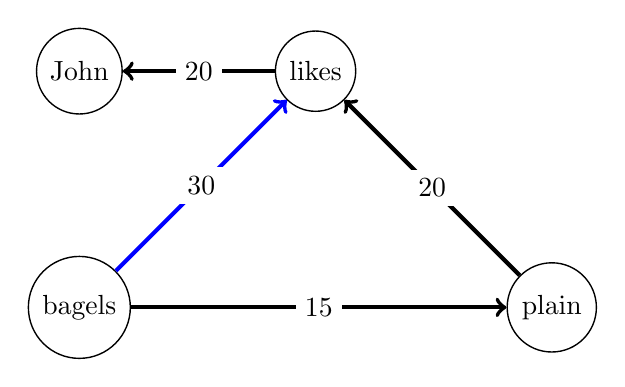
\begin{tikzpicture}
 \SetUpEdge[lw         = 1.5pt,
            color      = black,
            labelcolor = white]
  \GraphInit[vstyle=Normal] 
  \SetGraphUnit{3}
  \tikzset{VertexStyle/.append  style={fill}}
  \Vertex{John}
  \SO(John){bagels} \EA(John){likes}  \SOEA(likes){plain}
  \tikzset{EdgeStyle/.style={->}}
  \Edge[label=$20$](likes)(John)
  \Edge[label=$20$](plain)(likes)
  \Edge[label=$15$](bagels)(plain)
  \tikzstyle{EdgeStyle}=[color=blue, style ={->}]
  \Edge[label=$30$](bagels)(likes)
\end{tikzpicture}

\item We note there is a cycle and choose to contract the nodes connected by the edge in blue. We call this group $w_j$ and recalculate its incoming and outgoing edges: \\

\begin{tabular}{|c|c|c|}
\hline
\textbf{Incoming} & likes $\rightarrow$ bagels & bagels $\rightarrow$ likes \\ \hline
root $\rightarrow$ & {\color{red}$15+30 = 45$} & $0+10 = 10$ \\ \hline
John $\rightarrow$ & {\color{red}$5+30 = 35$} & $15+10 = 25$ \\ \hline
plain $\rightarrow$ & {\color{red}$20+30 = 50$} & $5+10 = 15$ \\ \hline 
\end{tabular} \\

\begin{tabular}{|c|c|c|}
\hline
\textbf{Outcoming} & likes & bagels \\ \hline
John $\leftarrow$ & {\color{red}$20$} & $5$ \\ \hline
plain $\leftarrow$ & $5$ & {\color{red}$15$} \\ \hline
\end{tabular} \\

\item The maximum incoming and outcoming edges per external node are marked in red. The new graph looks as follows:

\begin{multicols}{2}
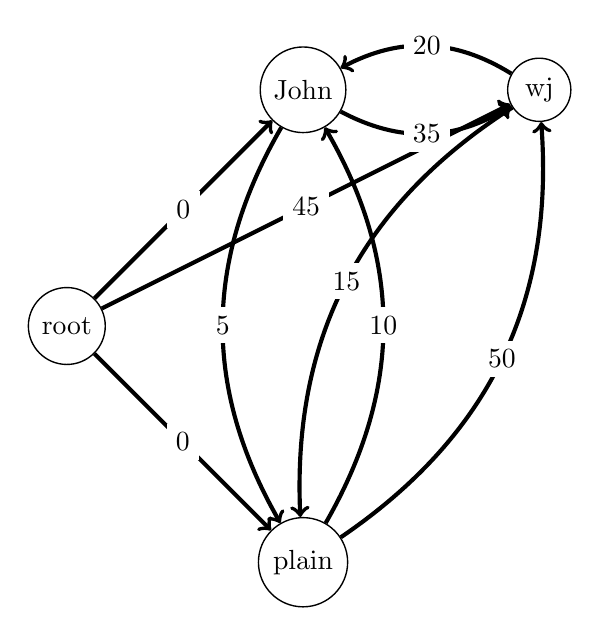
\begin{tikzpicture}
 \SetUpEdge[lw         = 1.5pt,
            color      = black,
            labelcolor = white]
  \GraphInit[vstyle=Normal] 
  \SetGraphUnit{3}
  \tikzset{VertexStyle/.append  style={fill}}
  \Vertex{root}
  \NOEA(root){John} \EA(John){wj}  \SOEA(root){plain}
  \tikzset{EdgeStyle/.style={->}}
  \Edge[label=$0$](root)(John)
  \Edge[label=$45$](root)(wj)
  \Edge[label=$0$](root)(plain)
  \Edge[label=$35$, style={bend right}](John)(wj)
  \Edge[label=$5$, style={bend right}](John)(plain)
  \Edge[label=$20$, style={bend right}](wj)(John)
  \Edge[label=$15$, style={bend right}](wj)(plain)
  \Edge[label=$10$, style={bend right}](plain)(John)
  \Edge[label=$50$, style={bend right}](plain)(wj)
\end{tikzpicture}

\begin{tabular}{|c|c|c|c|c|}
\hline
 & root & John & wj & plain \\ \hline
John & $0$ & - & $20$ & $10$ \\ \hline
wj & $45$ & $35$ & - & $50$ \\ \hline
plain & $0$ & $5$ & $15$ & - \\ \hline
\end{tabular} \\
\end{multicols}

\item We apply CLE recursively and go back to a) with the new graph as basis

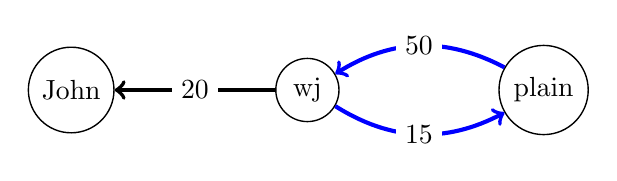
\begin{tikzpicture}
 \SetUpEdge[lw         = 1.5pt,
            color      = black,
            labelcolor = white]
  \GraphInit[vstyle=Normal] 
  \SetGraphUnit{3}
  \tikzset{VertexStyle/.append  style={fill}}
  \Vertex{John}
  \EA(John){wj}  \EA(wj){plain}
  \tikzset{EdgeStyle/.style={->}}
  \Edge[label=$20$](wj)(John)
  \tikzstyle{EdgeStyle}=[color=blue, style ={->}]
  \Edge[label=$50$, style={bend right}](plain)(wj)
  \Edge[label=$15$, style={bend right}](wj)(plain)
\end{tikzpicture}

\item Again, we have a cycle. We contract the nodes selected in blue, call it $w_k$ and recalculate the incoming and outgoing nodes. \\

\begin{tabular}{|c|c|c|}
\hline
\textbf{Incoming} & wj $\rightarrow$ plain & plain $\rightarrow$ wj \\ \hline
root $\rightarrow$ & {\color{red}$45+15 = 60$} & $0+50 = 50$ \\ \hline
John $\rightarrow$ & $35+15 = 50$ & {\color{red}$5+50 = 55$} \\ \hline 
\end{tabular} \\

\begin{tabular}{|c|c|c|}
\hline
\textbf{Outcoming} & wj & plain \\ \hline
John $\leftarrow$ & {\color{red}$20$} & $0$ \\ \hline
\end{tabular} \\

\item The resulting graph is:

\begin{multicols}{2}
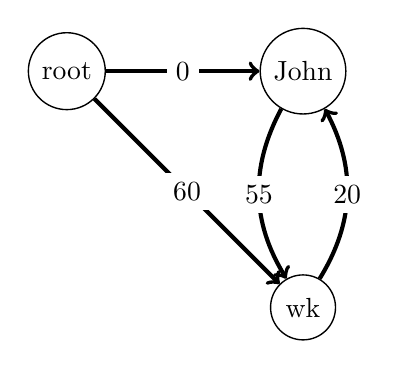
\begin{tikzpicture}
 \SetUpEdge[lw         = 1.5pt,
            color      = black,
            labelcolor = white]
  \GraphInit[vstyle=Normal] 
  \SetGraphUnit{3}
  \tikzset{VertexStyle/.append  style={fill}}
  \Vertex{root}
  \EA(root){John} \SOEA(root){wk}
  \tikzset{EdgeStyle/.style={->}}
  \Edge[label=$0$](root)(John)
  \Edge[label=$60$](root)(wk)
  \Edge[label=$55$, style={bend right}](John)(wk)
  \Edge[label=$20$, style={bend right}](wk)(John)
\end{tikzpicture}

\begin{tabular}{|c|c|c|c|}
\hline
 & root & John & wk \\ \hline
John & $0$ & - & $20$ \\ \hline
wk & $60$ & $55$ & - \\ \hline
\end{tabular} \\
\end{multicols}

\item Going back to a) once more:

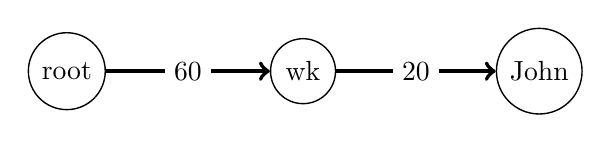
\begin{tikzpicture}
 \SetUpEdge[lw         = 1.5pt,
            color      = black,
            labelcolor = white]
  \GraphInit[vstyle=Normal] 
  \SetGraphUnit{3}
  \tikzset{VertexStyle/.append  style={fill}}
  \Vertex{wk}
  \WE(wk){root}  \EA(wk){John}
  \tikzset{EdgeStyle/.style={->}}
  \Edge[label=$20$](wk)(John)
  \Edge[label=$60$](root)(wk)
\end{tikzpicture}

\item Since there are no more cycles, we are done.

\end{enumerate}

\item Show the resulting MST \\

We interpret the previous graph and reconstruct it. Regarding wk outgoing edges, we backtrack that wk $\rightarrow$ John comes from wj $\rightarrow$ likes $\rightarrow$ John. Thus we include \textbf{likes $\rightarrow$ John}. \\

Regarding incoming edges, we backtrack that root $\rightarrow$ wk comes from root $\rightarrow$ wj $\rightarrow$ plain. On the one hand, root $\rightarrow$ wj comes from root $\rightarrow$ likes $\rightarrow$ bagels. 
On the other hand, wj $\rightarrow$ plain comes from bagels $\rightarrow$ plain. Thus we include \textbf{root $\rightarrow$ likes}, \textbf{likes $\rightarrow$ bagels}, and \textbf{bagels $\rightarrow$ plain}

\begin{tikzpicture}
 \SetUpEdge[lw         = 1.5pt,
            color      = black,
            labelcolor = white]
  \GraphInit[vstyle=Normal] 
  \SetGraphUnit{3}
  \tikzset{VertexStyle/.append  style={fill}}
  \Vertex{John} 
  \NO(likes){root} \SO(likes){bagels} \EA(John){likes}  \SOWE(likes){plain}
  \tikzset{EdgeStyle/.style={->}}
  \Edge[label=$15$](root)(likes)
  \Edge[label=$20$](likes)(John)
  \Edge[label=$30$](likes)(bagels)
  \Edge[label=$15$](bagels)(plain)
\end{tikzpicture}

\end{enumerate}
\end{exercise}
 
\begin{exercise}{5} Dependency parsing: Transition-based \\
Consider the sentence: \textbf{A koala eats leafs and barks}
\begin{enumerate}[label=(\alph*)]

\item Will a transition-based dependency parser be able to correctly predict this structure? \\ 
No. As seen in the next table, this transition-based dependency parser is not able to correctly predict this structure. \\ 

\begin{tabular}{|p{35mm}|p{35mm}|p{35mm}|p{40mm}|} \hline
\textbf{Transition} & \textbf{Stack} & \textbf{Buffer} & \textbf{Arc set} \\ \hline
- & [ROOT] & A koala eats leafs and barks & $\emptyset$ \\ \hline
SHIFT & [ROOT A] & koala eats leafs and barks & $\emptyset$ \\ \hline
SHIFT & [ROOT A koala] & eats leafs and barks & $\emptyset$ \\ \hline
LEFT-ARC(det) & [ROOT koala] & eats leafs and barks & A $\cup$ det(koala, A) \\ \hline
SHIFT & [ROOT koala eats] & leafs and barks & A \\ \hline
LEFT-ARC(nsubj) & [ROOT eats] & leafs and barks & A $\cup$ nsubj(eats, koala) \\ \hline
{\color{red}RIGHT-ARC(root)} & {\color{red}[ROOT]} & {\color{red}leafs and barks} & {\color{red}A $\cup$ root(root, eats)} \\ \hline
SHIFT & [ROOT leafs] & and barks & A \\ \hline
SHIFT & [ROOT leafs and] & barks & A \\ \hline
RIGHT-ARC(cc) & [ROOT leafs] & barks & A $\cup$ cc(leafs, and) \\ \hline
SHIFT & [ROOT leafs barks] & $\emptyset$ & A \\ \hline
RIGHT-ARC(conj) & [ROOT leafs] & $\emptyset$ & A $\cup$ conj(leafs, barks) \\ \hline
\end{tabular} \\

\item If there is a mistake, state what was the mistake \\
The arc-standard parser finds all but one arc: dobj(eats, leafs). The error arises in the configuration highlighted in {\color{red}red}, where the parser eliminates the word \textit{eats}, thus eliminating the possibility to connect \textit{eats} to \textit{leafs}. This error arises because the parser only performs local decisions, thus being ignorant to global structures.

\end{enumerate}
\end{exercise} 

\begin{exercise}{6} CCG
\begin{enumerate}[label=(\alph*), leftmargin=0mm]

\item Derive \textbf{The company added four Boeing-747s to the two units in 1994} \\

\begin{tabular}{@{}P{6.5mm}P{14mm}P{22mm}P{6.5mm}P{11.5mm}P{8.5mm}P{6.5mm}P{5.5mm}P{7.5mm}P{27mm}P{7mm}}
\textit{The} & \textit{company} & \textit{added} & \textit{four} & \textit{Boeing-747s} & \textit{to} & \textit{the} & \textit{two} & \textit{units} & \textit{in} & \textit{1994} \\
\tline{NP/N}{5.5mm} & \tline{N}{13mm} & \tline{((S\textbackslash NP)/PP)/NP}{21mm} & \tline{NP/N}{5.5mm} & \tline{N}{10.5mm} & \tline{PP/NP}{7.5mm} & \tline{NP/N}{6mm} & \tline{N/N}{4.5mm} & \tline{N}{6.5mm} & \tline{((S\textbackslash NP)\textbackslash (S\textbackslash NP))/NP}{26mm} & \tline{NP}{6mm} \\
\fline{NP}{19.5mm} & & & \fline{NP}{17mm} & & & & \fline{N}{12mm} & & \fline{(S\textbackslash NP)\textbackslash (S\textbackslash NP)}{33mm} & \\
& & & & & & \fline{NP}{22mm} & & & & \\
& & \fline{(S\textbackslash NP)/PP}{45mm} & & & \fline{PP}{35mm} & & & & & \\
& & \fline{(S\textbackslash NP)}{87mm} & & & & & & & & \\
& & \bline{S\textbackslash NP}{130mm} & & & & & & & & \\
\bline{S}{160mm} & & & & & & & & & & \\
\end{tabular} \\

\item Derive noun phrases for \textbf{the company which added four Boeing-747s to the two units in 1994} and \textbf{the four Boeing-747s which the company added to the two units in 1994} \\

First case: \\

\begin{tabular}{@{}P{6mm}P{13mm}P{20mm}P{22mm}P{6.5mm}P{11.5mm}P{8.5mm}P{6.5mm}P{5.5mm}P{7mm}P{27mm}P{7mm}}
\textit{the} & \textit{company} & \textit{which} & \textit{added} & \textit{four} & \textit{Boeing-747s} & \textit{to} & \textit{the} & \textit{two} & \textit{units} & \textit{in} & \textit{1994} \\
\tline{NP/N}{5.5mm} & \tline{N}{13mm} & \tline{(NP/(S\textbackslash NP))\textbackslash NP}{18mm} & \tline{((S\textbackslash NP)/PP)/NP}{21mm} & \tline{NP/N}{5.5mm} & \tline{N}{10.5mm} & \tline{PP/NP}{7.5mm} & \tline{NP/N}{6mm} & \tline{N/N}{4.5mm} & \tline{N}{6.5mm} & \tline{((S\textbackslash NP)\textbackslash (S\textbackslash NP))/NP}{26mm} & \tline{NP}{6mm} \\
\fline{NP}{19.5mm} & & & & \fline{NP}{17mm} & & & & \fline{N}{12mm} & & \fline{(S\textbackslash NP)\textbackslash (S\textbackslash NP)}{33mm} & \\
\bline{NP/(S\textbackslash NP)}{43mm} & & & & & & & \fline{NP}{22mm} & & & & \\
& & & \fline{(S\textbackslash NP)/PP}{45mm} & & & \fline{PP}{35mm} & & & & & \\
& & & \fline{(S\textbackslash NP)}{87mm} & & & & & & & & \\
& & & \bline{S\textbackslash NP}{130mm} & & & & & & & & \\
\fline{NP}{180mm} & & & & & & & & & & \\
\end{tabular} \\

Here, \textit{which} has the lexical category (NP/(S\textbackslash NP))\textbackslash NP. If we interpret S\textbackslash NP as a VP, then the category for \textit{which} can be interpret as: \\

\textsc{Given a noun phrase before, and a verb phrase after, } \textit{which} \textsc{will produce a noun phrase}.\\


In order to derive the second noun phrase we had to make a couple assumptions. First, the category for \textit{added} was changed from ((S\textbackslash NP)/PP)/NP to ((S\textbackslash NP)/PP). We believe that for this word, both are lexical categories valid. Second, the category for \textit{four} was changed from NP/N to N/N. This change was inspired by looking at the category of \textit{two}, which is equivalent to \textit{four}. \\

\begin{tabular}{@{}P{8mm}@{}P{9mm}@{}P{17mm}@{}P{25mm}@{}P{9mm}@{}P{15mm}@{}P{24mm}@{}P{13mm}@{}P{8mm}@{}P{8mm}@{}P{9mm}@{}P{28mm}@{}P{8mm}}
\textit{the} & \textit{four} & \textit{Boeing-747s} & \textit{which} & \textit{the} & \textit{company} & \textit{added} & \textit{to} & \textit{the} & \textit{two} & \textit{units} & \textit{in} & \textit{1994} \\
\tline{NP/N}{6mm} & \tline{N/N}{7mm} & \tline{N}{11mm} & \tline{(NP/S)\textbackslash NP}{18mm} & \tline{NP/N}{6mm} & \tline{N}{13mm} & \tline{(S\textbackslash NP)/PP}{15mm} & \tline{PP/NP}{8mm} & \tline{NP/N}{6mm} & \tline{N/N}{6mm} & \tline{N}{7mm} & \tline{((S\textbackslash NP)\textbackslash (S\textbackslash NP))/NP}{26mm} & \tline{NP}{6mm} \\
& \fline{N}{19.5mm} & & & \fline{NP}{17mm} & & & & & \fline{N}{12mm} & & \fline{(S\textbackslash NP)\textbackslash (S\textbackslash NP)}{33mm} & \\
\fline{NP}{28mm} & & & & & & & & \fline{NP}{22mm} & & & & \\
\bline{NP/S}{52mm} & & & & & & & \fline{PP}{35mm} & & & & \\
& & & & & & \fline{(S\textbackslash NP)}{50mm} & & & & & \\
& & & & & & \bline{S\textbackslash NP}{93mm} & & & & & \\
& & & & \bline{S}{118mm} & & & & & & & \\
\fline{NP}{178mm} & & & & & & & & & & & \\
\end{tabular} \\

Here, \textit{which} has the lexical category (NP/S)\textbackslash NP. This time the category for \textit{which} can be interpret as: \\

\textsc{Given a noun phrase before, and a sentence after, } \textit{which} \textsc{will produce a noun phrase}.\\

\item Dutch sentence that is non-context free \\

As taken from \cite{steedman2011combinatory}

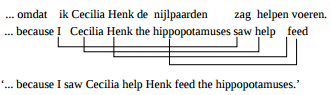
\includegraphics{dutch_dependency.png}

Where \textit{zag}, the verb, is separated from \textit{ik}, its subject, by  4 words forming an argument by themselves. 

\end{enumerate}
\end{exercise}
 
% --------------------------------------------------------------
%     You don't have to mess with anything below this line.
% --------------------------------------------------------------
\bibliographystyle{plain}
\bibliography{mybib} 
 
 
\end{document}